\chapter{Discussion}

\todo{
	**Things to avoid
	2Hyping findings-
	3Interpreting beyond what can be justified-
	4Extend in tangential topics-}

1-Intro - to be written when the section is more mature

2-What have we done:  a paragraph or two explaining the major findings and why are important.

\section{Problems and limitations}
3-Explain main problems and limitations and how are handled. Be succinct, be frank but no apologetic. Explain implications of limitations.
\subsection{Layout improvement procedure and issues, title to be improved}
opto <--x-->driver voltage levels?

inductor saturation and so

pcb hot points

...
\subsection{output cap?}
\subsection{MPPT drifting and improvement and limitations of final control algorithm}
The development of an embedded control system requires the proper working of an algorithm. During the development process, the engineer might find that the code doesn't behave as intended. A common way of supporting the debugging process consists on the use of breakpoints, where the code is stopped and the variables' value might be read. However, as this feature is not supported by the used platform, and in the case of controlling physical systems its use would be limited to simulation, alternative techniques had to be used. The adopted approach consisted on outputting the FSMs state and relevant values for the current state at every code execution loop. The 'Timestamp' field is specially important during simulation in order to track specific events at determined times. See figure \ref{console_output}.

\begin{figure}[htbp]
	\begin{center}
		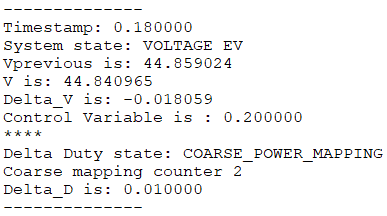
\includegraphics[width=0.5\textwidth]{../Pictures/P1/Discussion/console_output.png}
		\caption{Console output.}
		\label{console_output}
	\end{center}	
\end{figure}

In initial implementations of the control algorithm, the voltage evaluation was performed in the state next to the duty cycle change. After this change, the system experiences a transient stage where the input voltage and inductor current evolve into the new steady state value. If these variables are read during the transient, the control might infer that the PV panel is in a location of the P-V curve different than where it actually is. The MPPT becomes noisier under this scenario. In order to address this issue, an additional waiting state was added to the FSM governing the system. Another solution to the issue would be to decrease the MPPT algorithm periodicity. However this solution would lead to a decrease in system's responsiveness. However this drawback might be bearable by implementing a voltage controller aside from the MPPT.  

limitations of MPPT

\subsection{software filtering}
Although the voltage and current measurement is filtered, the signal read by the control system was noisy. This noise affected the MPPT algorithm disturbing its ability to reach the MPP. Such noise might have different sources within a lab with such a big amount of hardware equipment. There are many techniques in order to address noise issues, the used technique consists on the use of digital filtering (LPF). This digital filter is a  simple code that performs the filtering at a given frequency. Being a first order filter, it was simple and fast to implement and test. 
..
.

filtering image result
\subsection{...}

\section{Future work}
4- Recommendations for future work. Make general statements. Items: a)what study is needed, b)Methods to be used, c)what is needed for that study.
\subsection{different mppt technique}
\subsection{V/I controller}
\subsection{switching frequency limitations}
\subsection{pcb possible improvements}
bootstrap, change driver to the A version due to voltage levels and then change the optocouupler to a quad version,...
\subsection{component price, system size, optimization needed}
\subsection{efficiency}
\subsection{...}




